\subsubsection{Types}
There are three different types of \acrshort{rnn}:
\begin{itemize}
    \item Many to One: From a sequence generate a vector. For example, rate from one to ten opinions on products written by customers.
    \item Many to many: From sequence to generate a sequence. For example, translate text from one language to another.
    \item One to many: From a single vector a sequence is generated. For example, a network specialized in describing the elements of an image.
\end{itemize}

\begin{figure}[H]
    \centering
    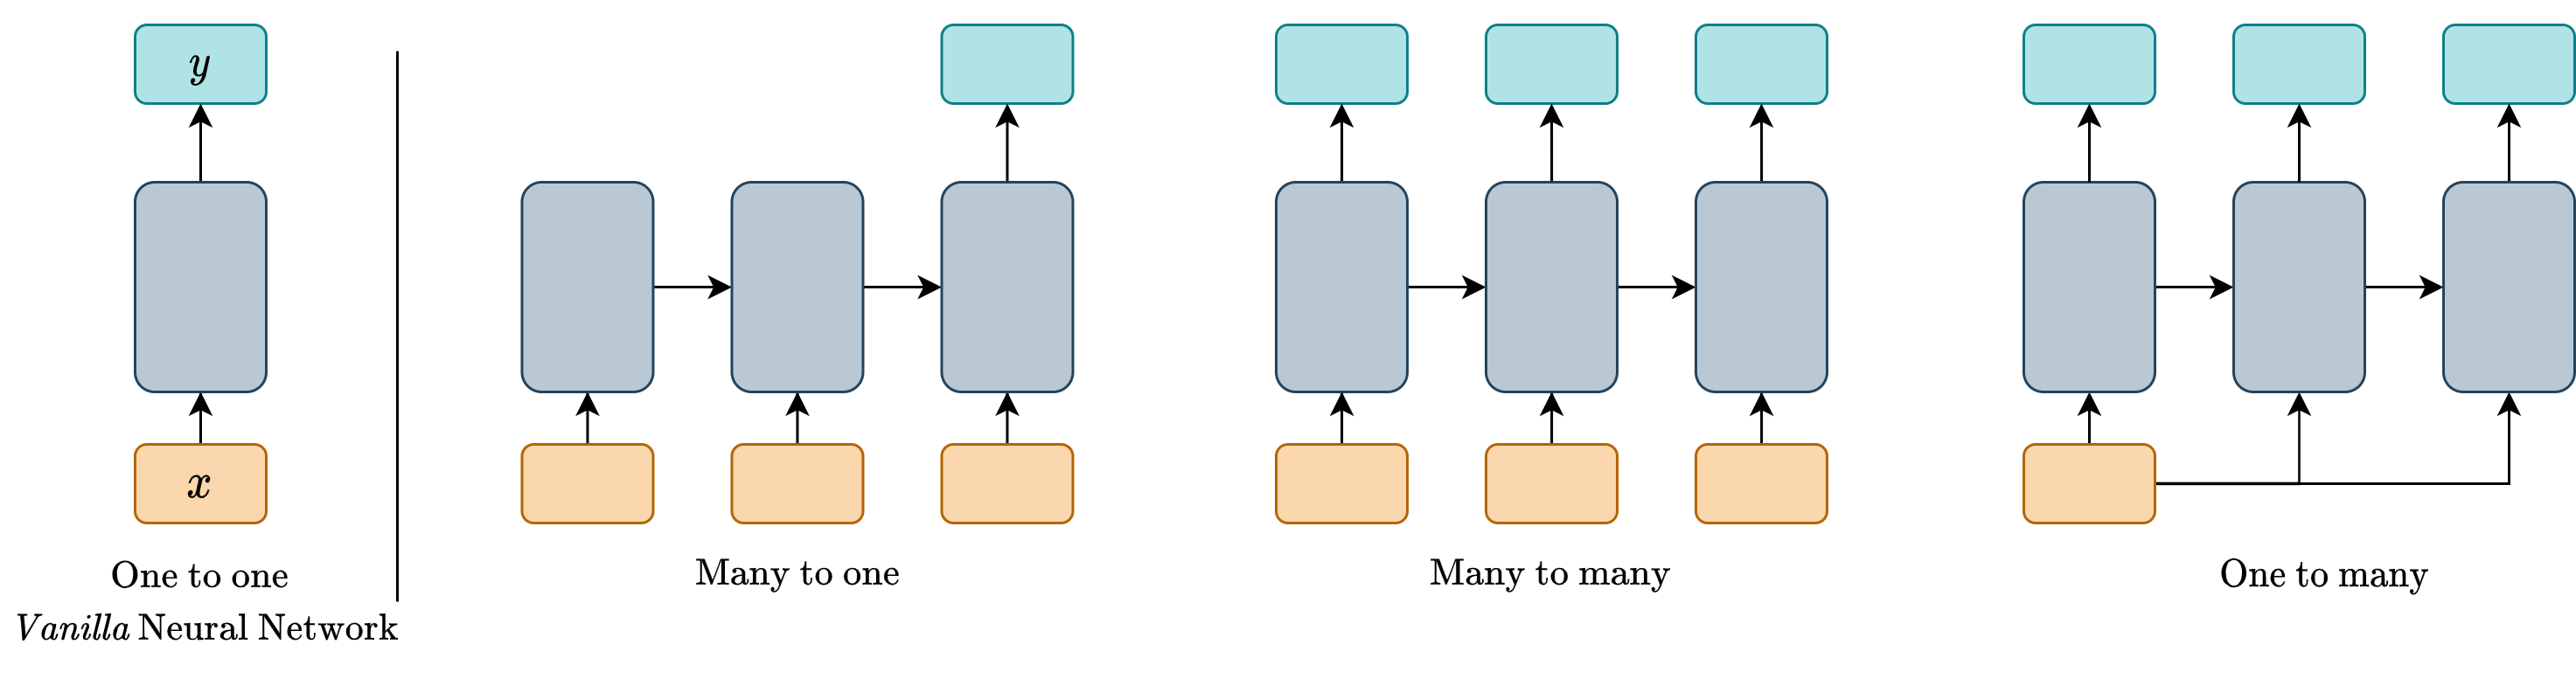
\includegraphics[width=14cm]{images/state-of-art/rnn/rnn-types.png}
    \caption{Operational representation of \acrshort{rnn} types}
    \label{fig:rnn_types}
\end{figure}
